\section{Blockchain}
\label{sec:blockchain-module}

Nel seguente capitolo viene descritto in maniera più approfondita il componente \textit{Blockchain}. In particolare, vengono analizzati gli smart contracts, i quali sono stati sviluppati utilizzando il framework \textit{Hardhat} e il linguaggio di programmazione \textit{Solidity} ma anche gli script utilizzati per l'automazione di alcune operazioni, i test effettuati e le possibili alternative.

\subsection{Smart contracts}
\label{sec:smart-contract-shopychange}

Per il corretto funzionamento del marketplace, sono stati sviluppati diversi smart contracts. In particolare, il contratto principale è \textit{ShopychangeMarketplace}, il quale si occupa di gestire la creazione, modifica, cancellazione e acquisto di una vendita. Inoltre, gestisce le \textit{royalty} e fornisce delle funzionalità di controllo per gli amministratori.

In aggiunta, il contratto \textit{ERC721 Factory} offre la possibilità di creazione di nuovi smart contracts di tipo \textit{ERC721} utilizzando un \textit{template} chiamato \textit{Boilerplate ERC721}. 

Infine, lo \textit{smart contract} \textit{Storage} viene utilizzato dagli utenti che non hanno necessità di creare una nuova collezione ma di generare un singolo asset.  

Nei prossimi capitoli verranno analizzati in dettaglio i contratti che compongono il marketplace. Di seguito, a figura \ref{fig:legenda}, è osservabile una legenda per la comprensione dei diagrammi.
\begin{figure}[H]
    \centering
    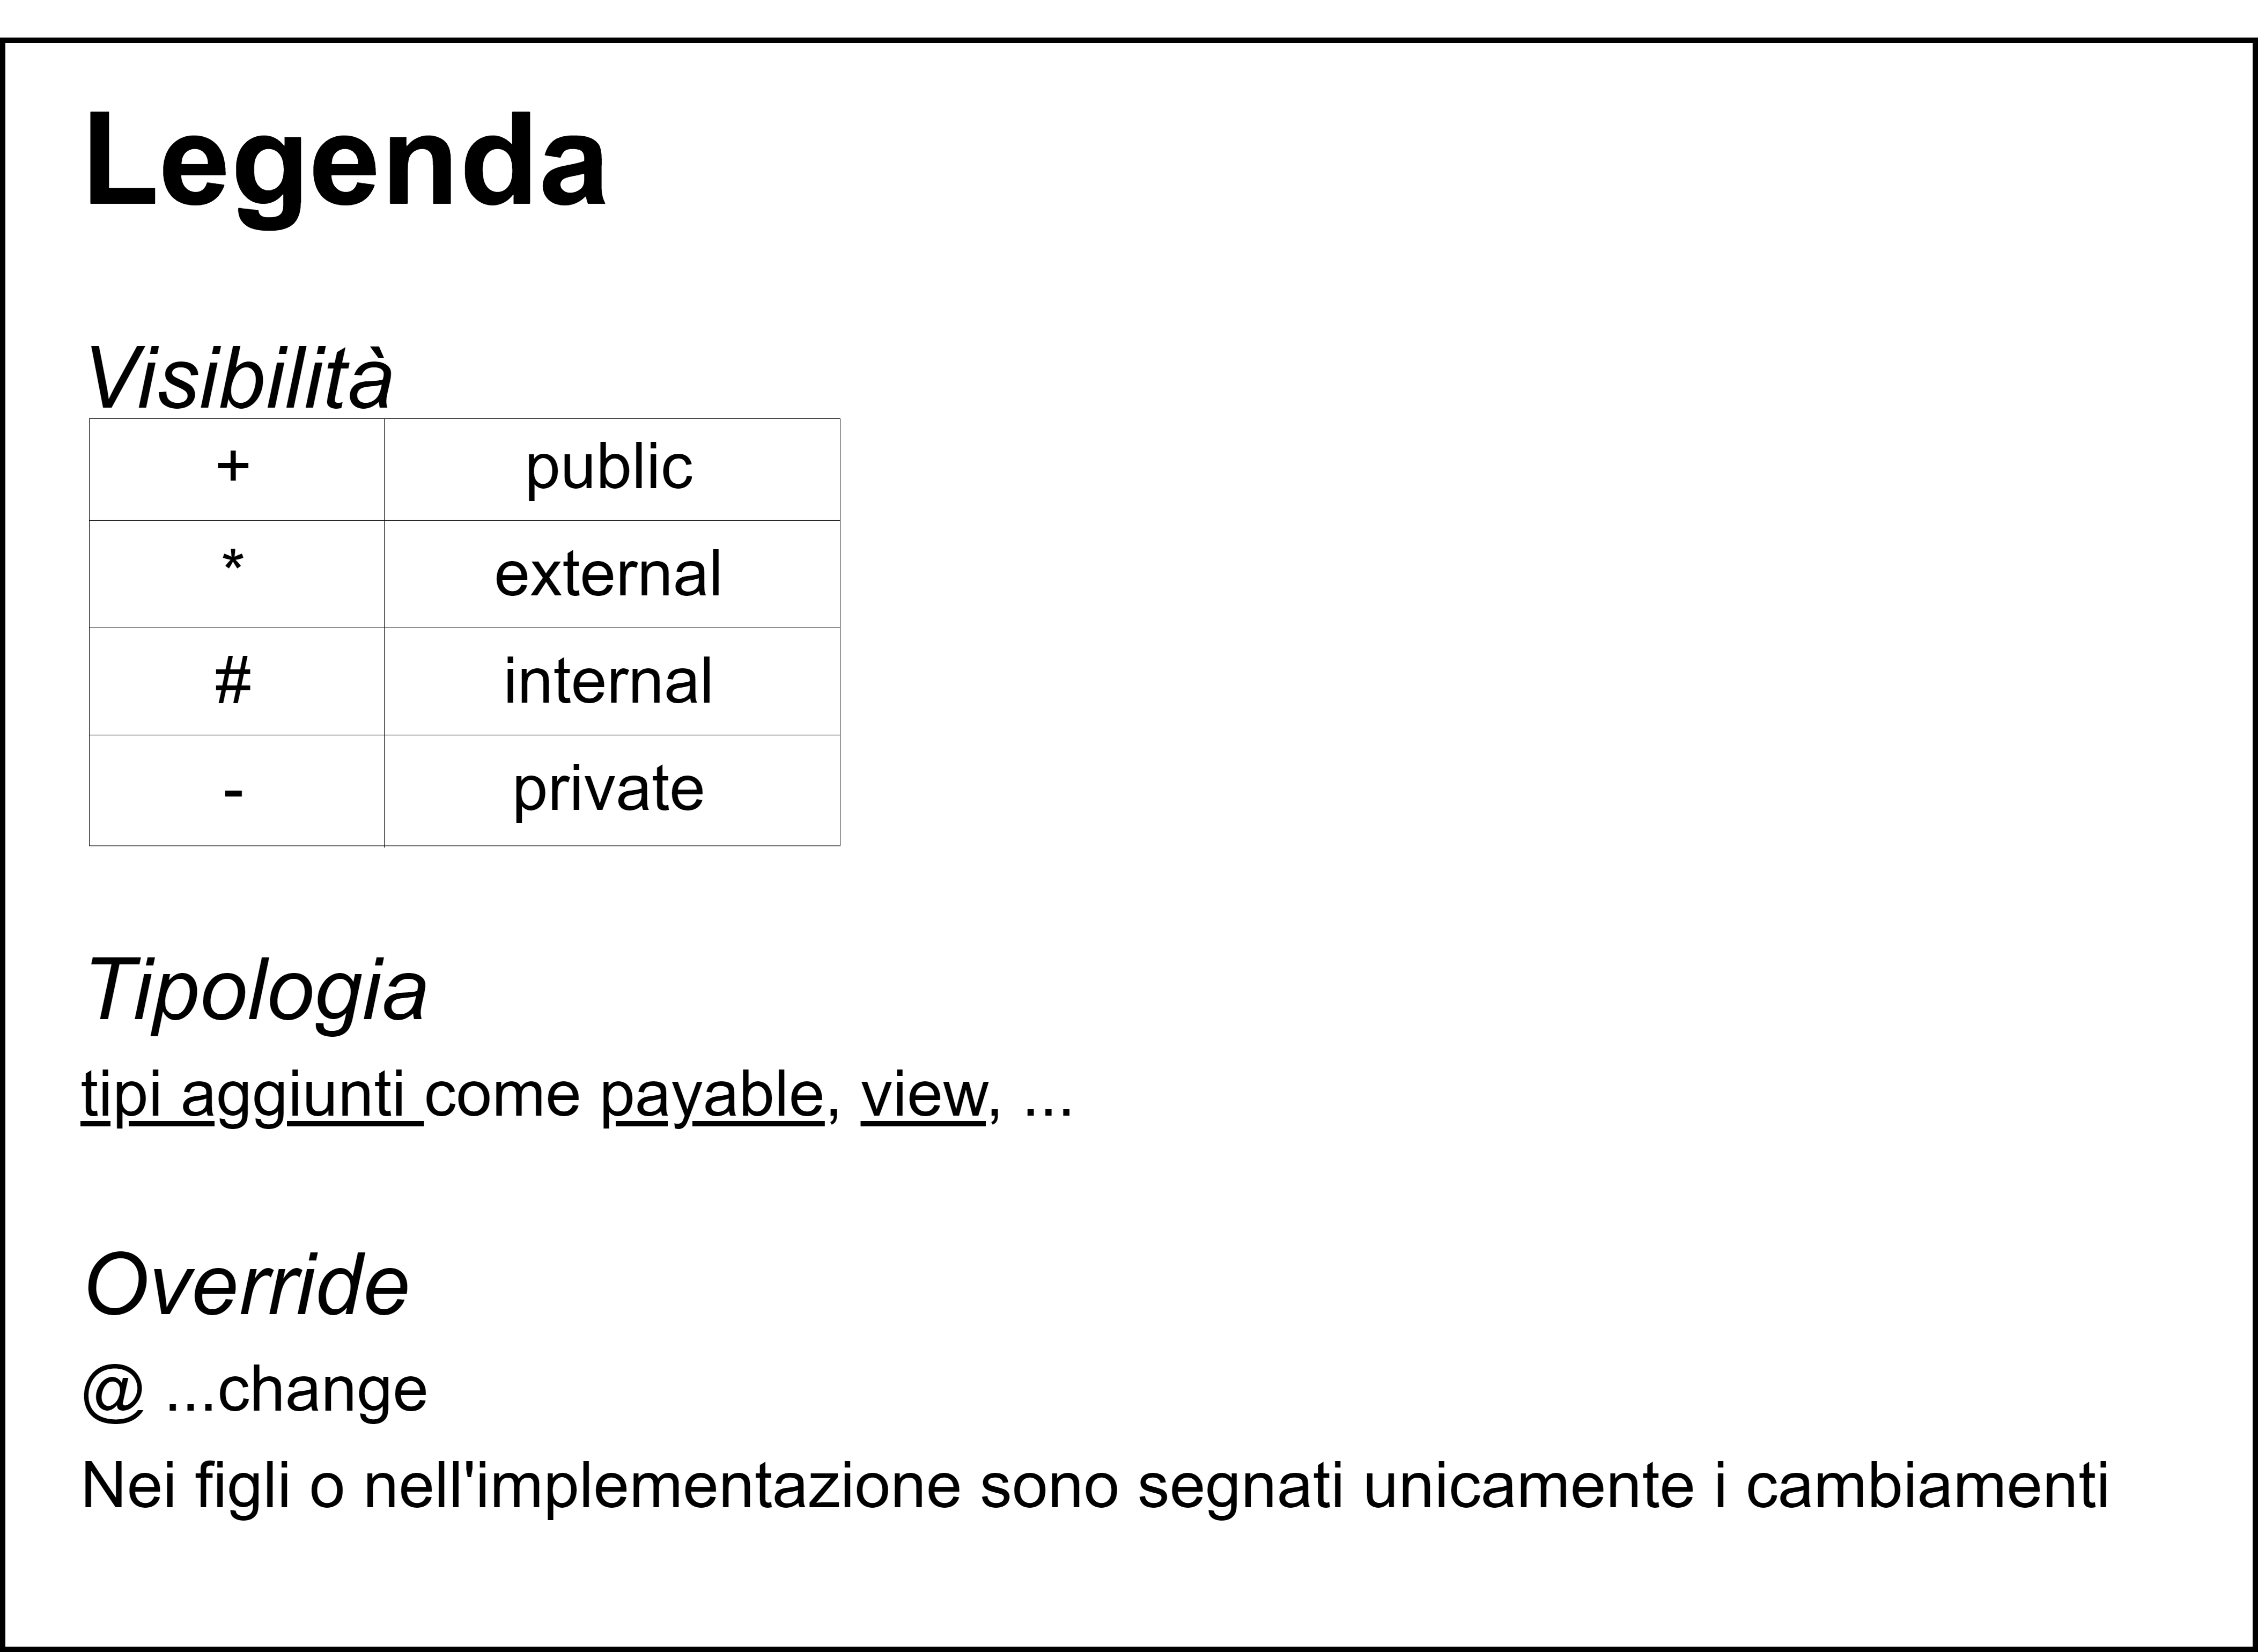
\includegraphics[width=0.8\textwidth]{images/blockchainContracts/LegendaBordo.png}
    \caption{Legenda Smart contracts}
    \label{fig:legenda}
\end{figure}

\subsubsection{Marketplace}

Il contratto \textit{core} del marketplace è \textit{ShopychangeMarketplace}. Per la sua realizzazione è stato deciso di utlizzare un approccio simile allo standard \textit{ERC721}, ovvero separando la logica in più contratti per facilitare la manutenzione, comprensione e testabilità del codice. Inoltre, grazie alla struttura a modelli è possibile decidere quali funzionalità abilitare o meno. Il contratto \textit{ShopychangeMarketplace} possiede tutte le funzionalità. La figura \ref{fig:marketplaceContract} mostra il diagramma UML del contratto.

\begin{figure}[H]
    \centering
    \includegraphics[width=1\textwidth]{images/blockchainContracts/ShopychangeMarketplaceReduced.png}
    \caption{Diagramma smart contract ShopychangeMarketplace}
    \label{fig:marketplaceContract}
\end{figure}


\paragraph{Fundamental}

Come si può osservare dalla figura \ref{fig:marketplaceFundamental}, il contratto \textit{MarketplaceFundamental} eredita dall'interfaccia \textit{IMarketplaceFundamental}. Questa interfaccia definisce le funzionalità obbligatorie del contratto \textit{Fundamental}, ovvero la creazione e acquisto di una vendita. Le informazioni relative alla vendita sono salvate in una struttura dati chiamata \textit{Sale}. Più in dettaglio, la struttura dati contiene le seguenti informazioni:

\begin{itemize}
    \item \textit{contractAddress}: indirizzo del contratto che rappresenta la collezione
    \item \textit{tokenId}: identificativo dell'asset all'interno della collezione
    \item \textit{price}: prezzo di vendita
    \item \textit{seller}: indirizzo del venditore
    \item \textit{status}: stato della vendita, può essere \textit{None} = 0 (Non presente nel marketplace), \textit{Cancelled} = 1 (Cancellata), \textit{Sold} = 2 (Venduta), \textit{Listed} = 3 (In vendita)
\end{itemize}

Gli attributi \textit{\_sales} e \textit{\_salesIds} presenti nel contratto \textit{MarketplaceFundamental} sono utilizzati per mantenere le informazioni relative alle vendite. In maniera più approfondita, \textit{\_sales} è una \textit{map} che associa ad ogni identificativo di una vendita la struttura dati \textit{Sale}. Mentre, \textit{\_salesIds} è un array che contiene gli identificativi delle vendite presenti nel marketplace. L'id in formato \textit{bytes32} è generato crittografando l'indirizzo del contratto e l'identificativo dell'asset, creando così un valore univoco per ogni vendita. L'id generato è ottenibile utilizzando la funzione \textit{getKey}. 

Nel momento in cui avviene la creazione di una vendita, lo smart contract controllerà che le informazioni fornite siano valevoli e che il chiamante sia effettivamente il possessore dell'asset. Un processo simili avviene anche all'acquisto del token, dove il contratto verifica che il \textit{seller} sia ancora il possessore. Maggiori dettagli su questa possibile situazioni sono presenti nel capitolo \hyperref[sec:controllo-integrita-nft-in-vendita]{\textit{Controllo integrità NFT in vendita}}.

Nel momento in cui avviene un acquisto, il metodo \textit{buy} eseguirà \textit{payShares}, questo meccanismo permetterà ai contratti figli di poter gestire le \textit{royalty} in maniera personalizzata. Maggiori informazioni nei capitoli \hyperref[sec:marketplace-earnable]{\textit{Earnable}} e \hyperref[sec:marketplace-royalty-applicable]{\textit{RoyaltyApplicable}}.

Infine, il contratto presenta alcune funzioni di tipo \textit{view}, le quali permettono di ottenere le vendite presenti nel marketplace.

\begin{figure}[H]
    \centering
    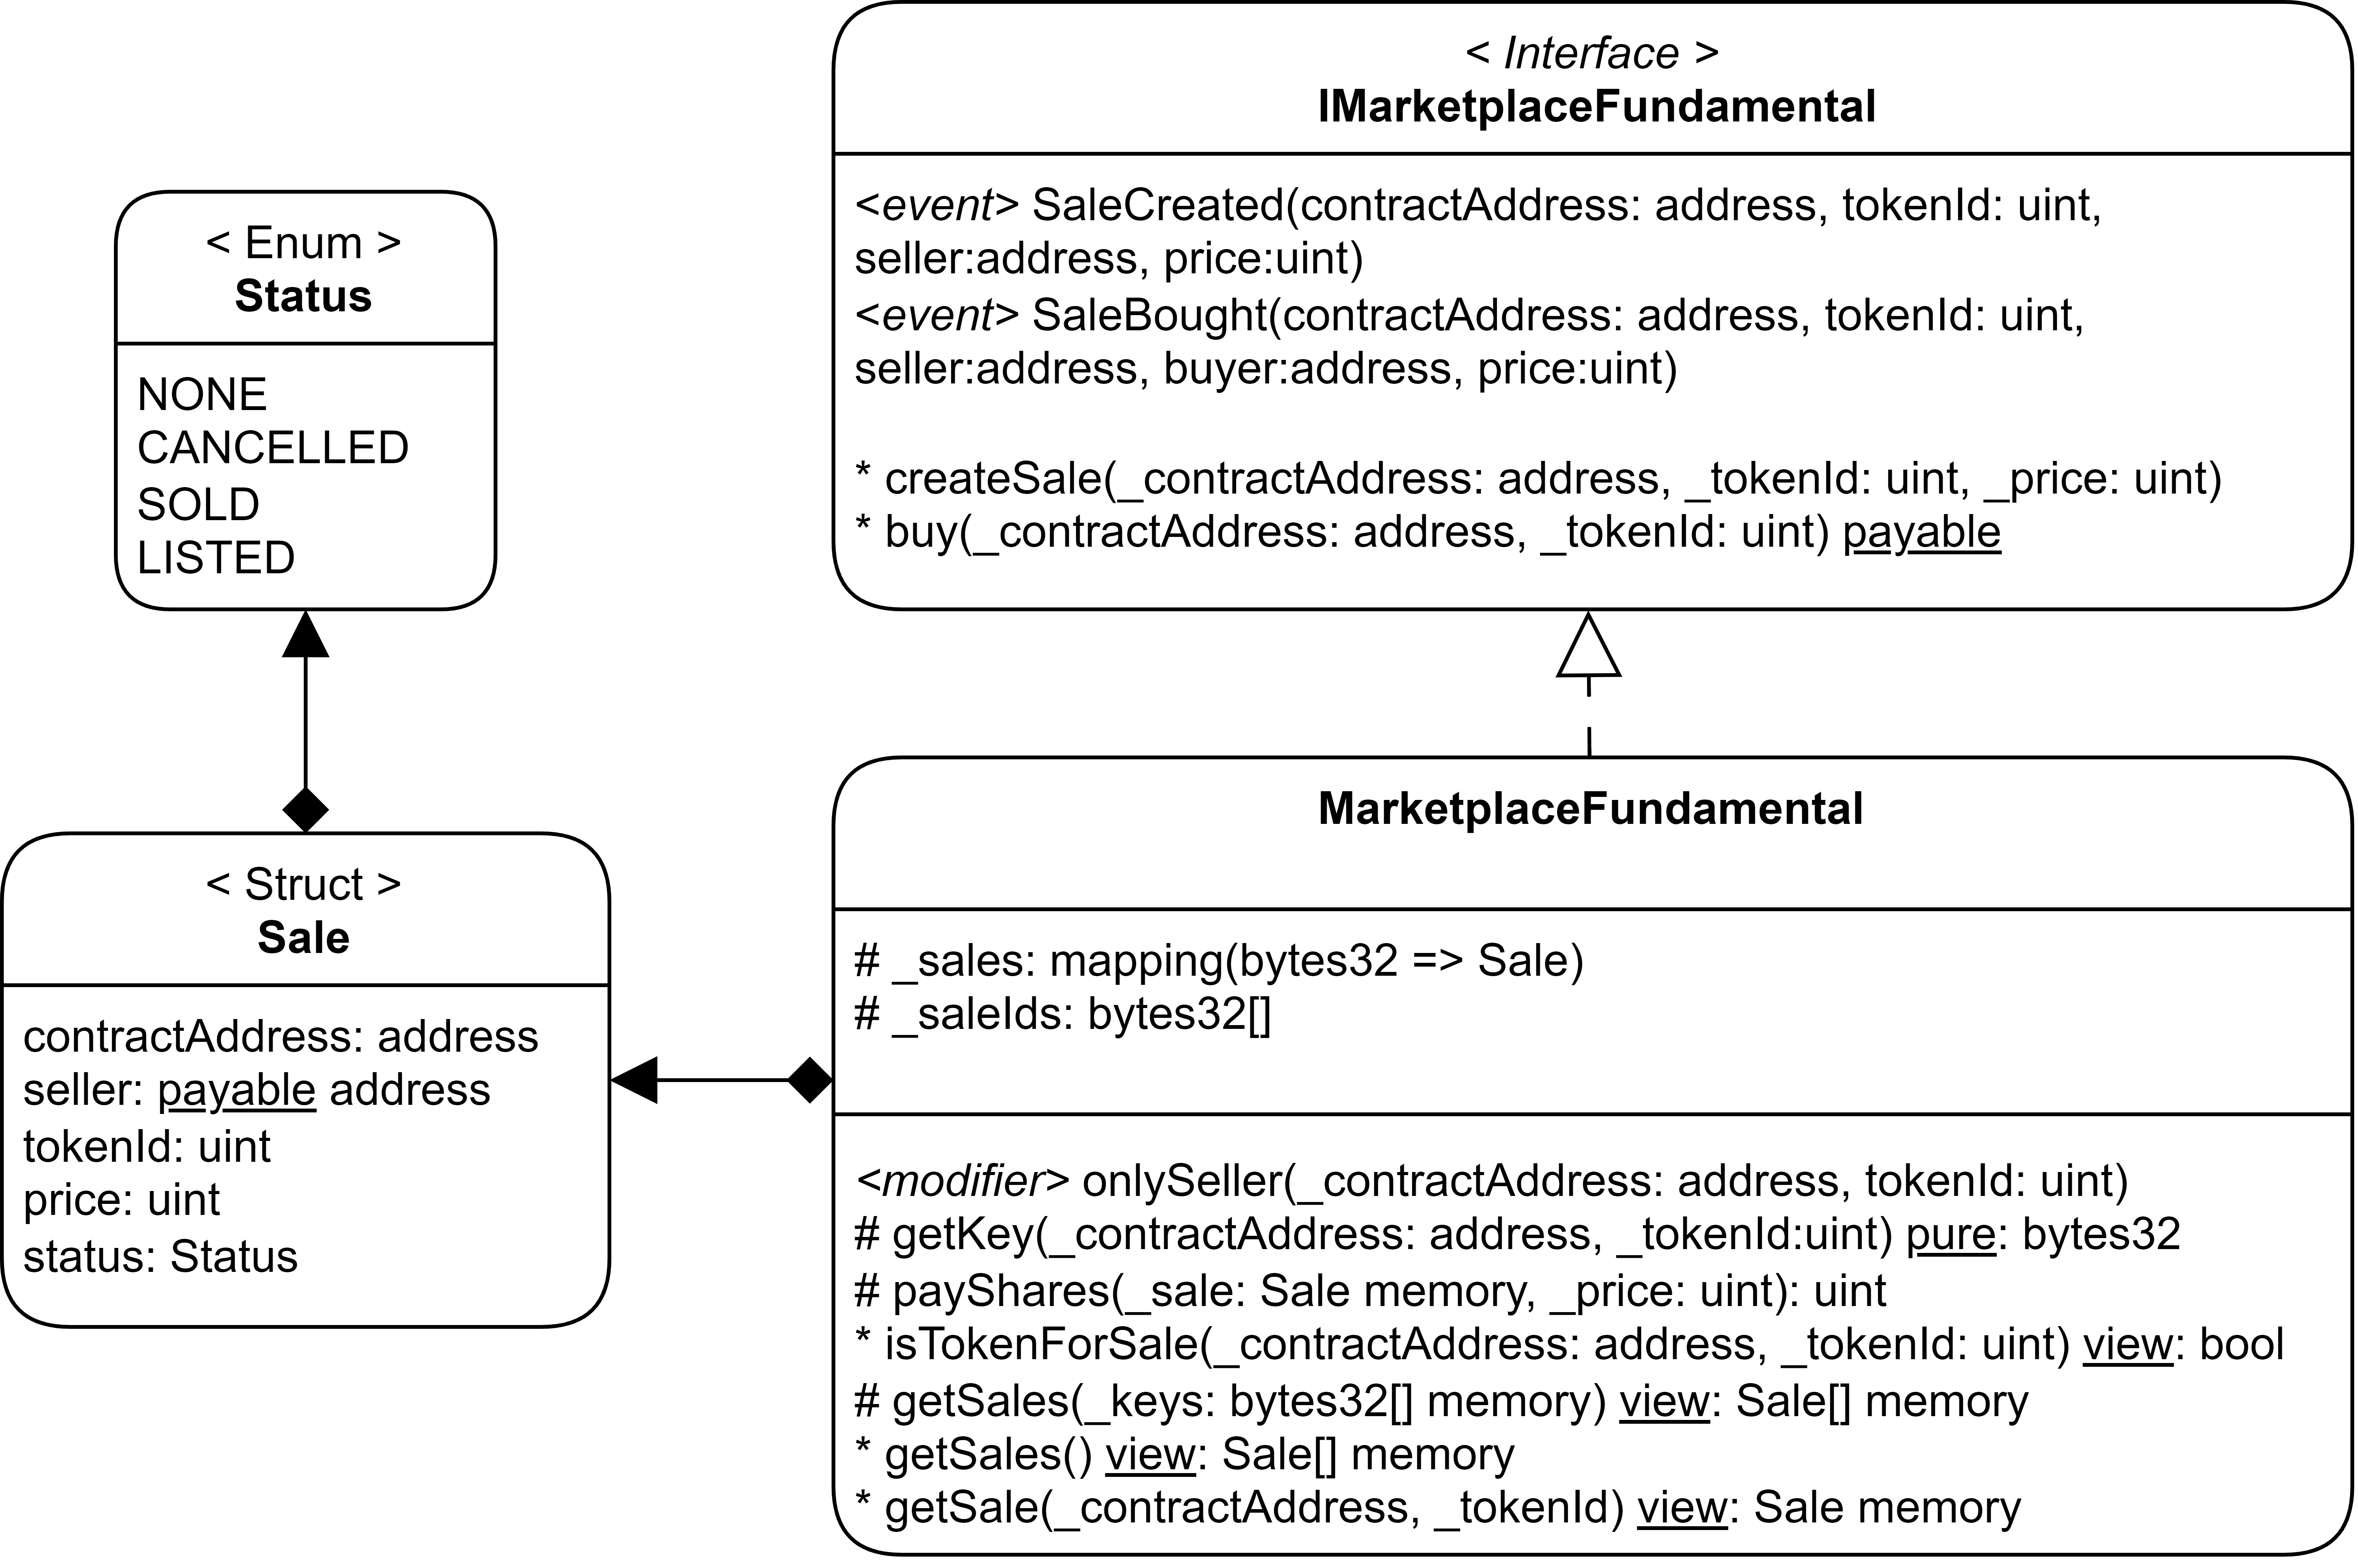
\includegraphics[width=1\textwidth]{images/blockchainContracts/MarketplaceFundamental.png}
    \caption{Marketplace Fundamental}
    \label{fig:marketplaceFundamental}
\end{figure}



\paragraph{Cancellable}
L'estensione \textit{Cancellable} permette la cancellazione di una vendita in corso. Nello specifico, il contratto \textit{MarketplaceCancellable} eredita da \textit{IMarketplaceCancellable} e \textit{MarketplaceFundamental}. Come visibile in figura \ref{fig:marketplaceCancellable} il contratto presenta la funzione \textit{cancelSale}, la quale è utilizzabile unicamente dal possessore dell'asset o dall'amministratore.

\begin{figure}[H]
    \centering
    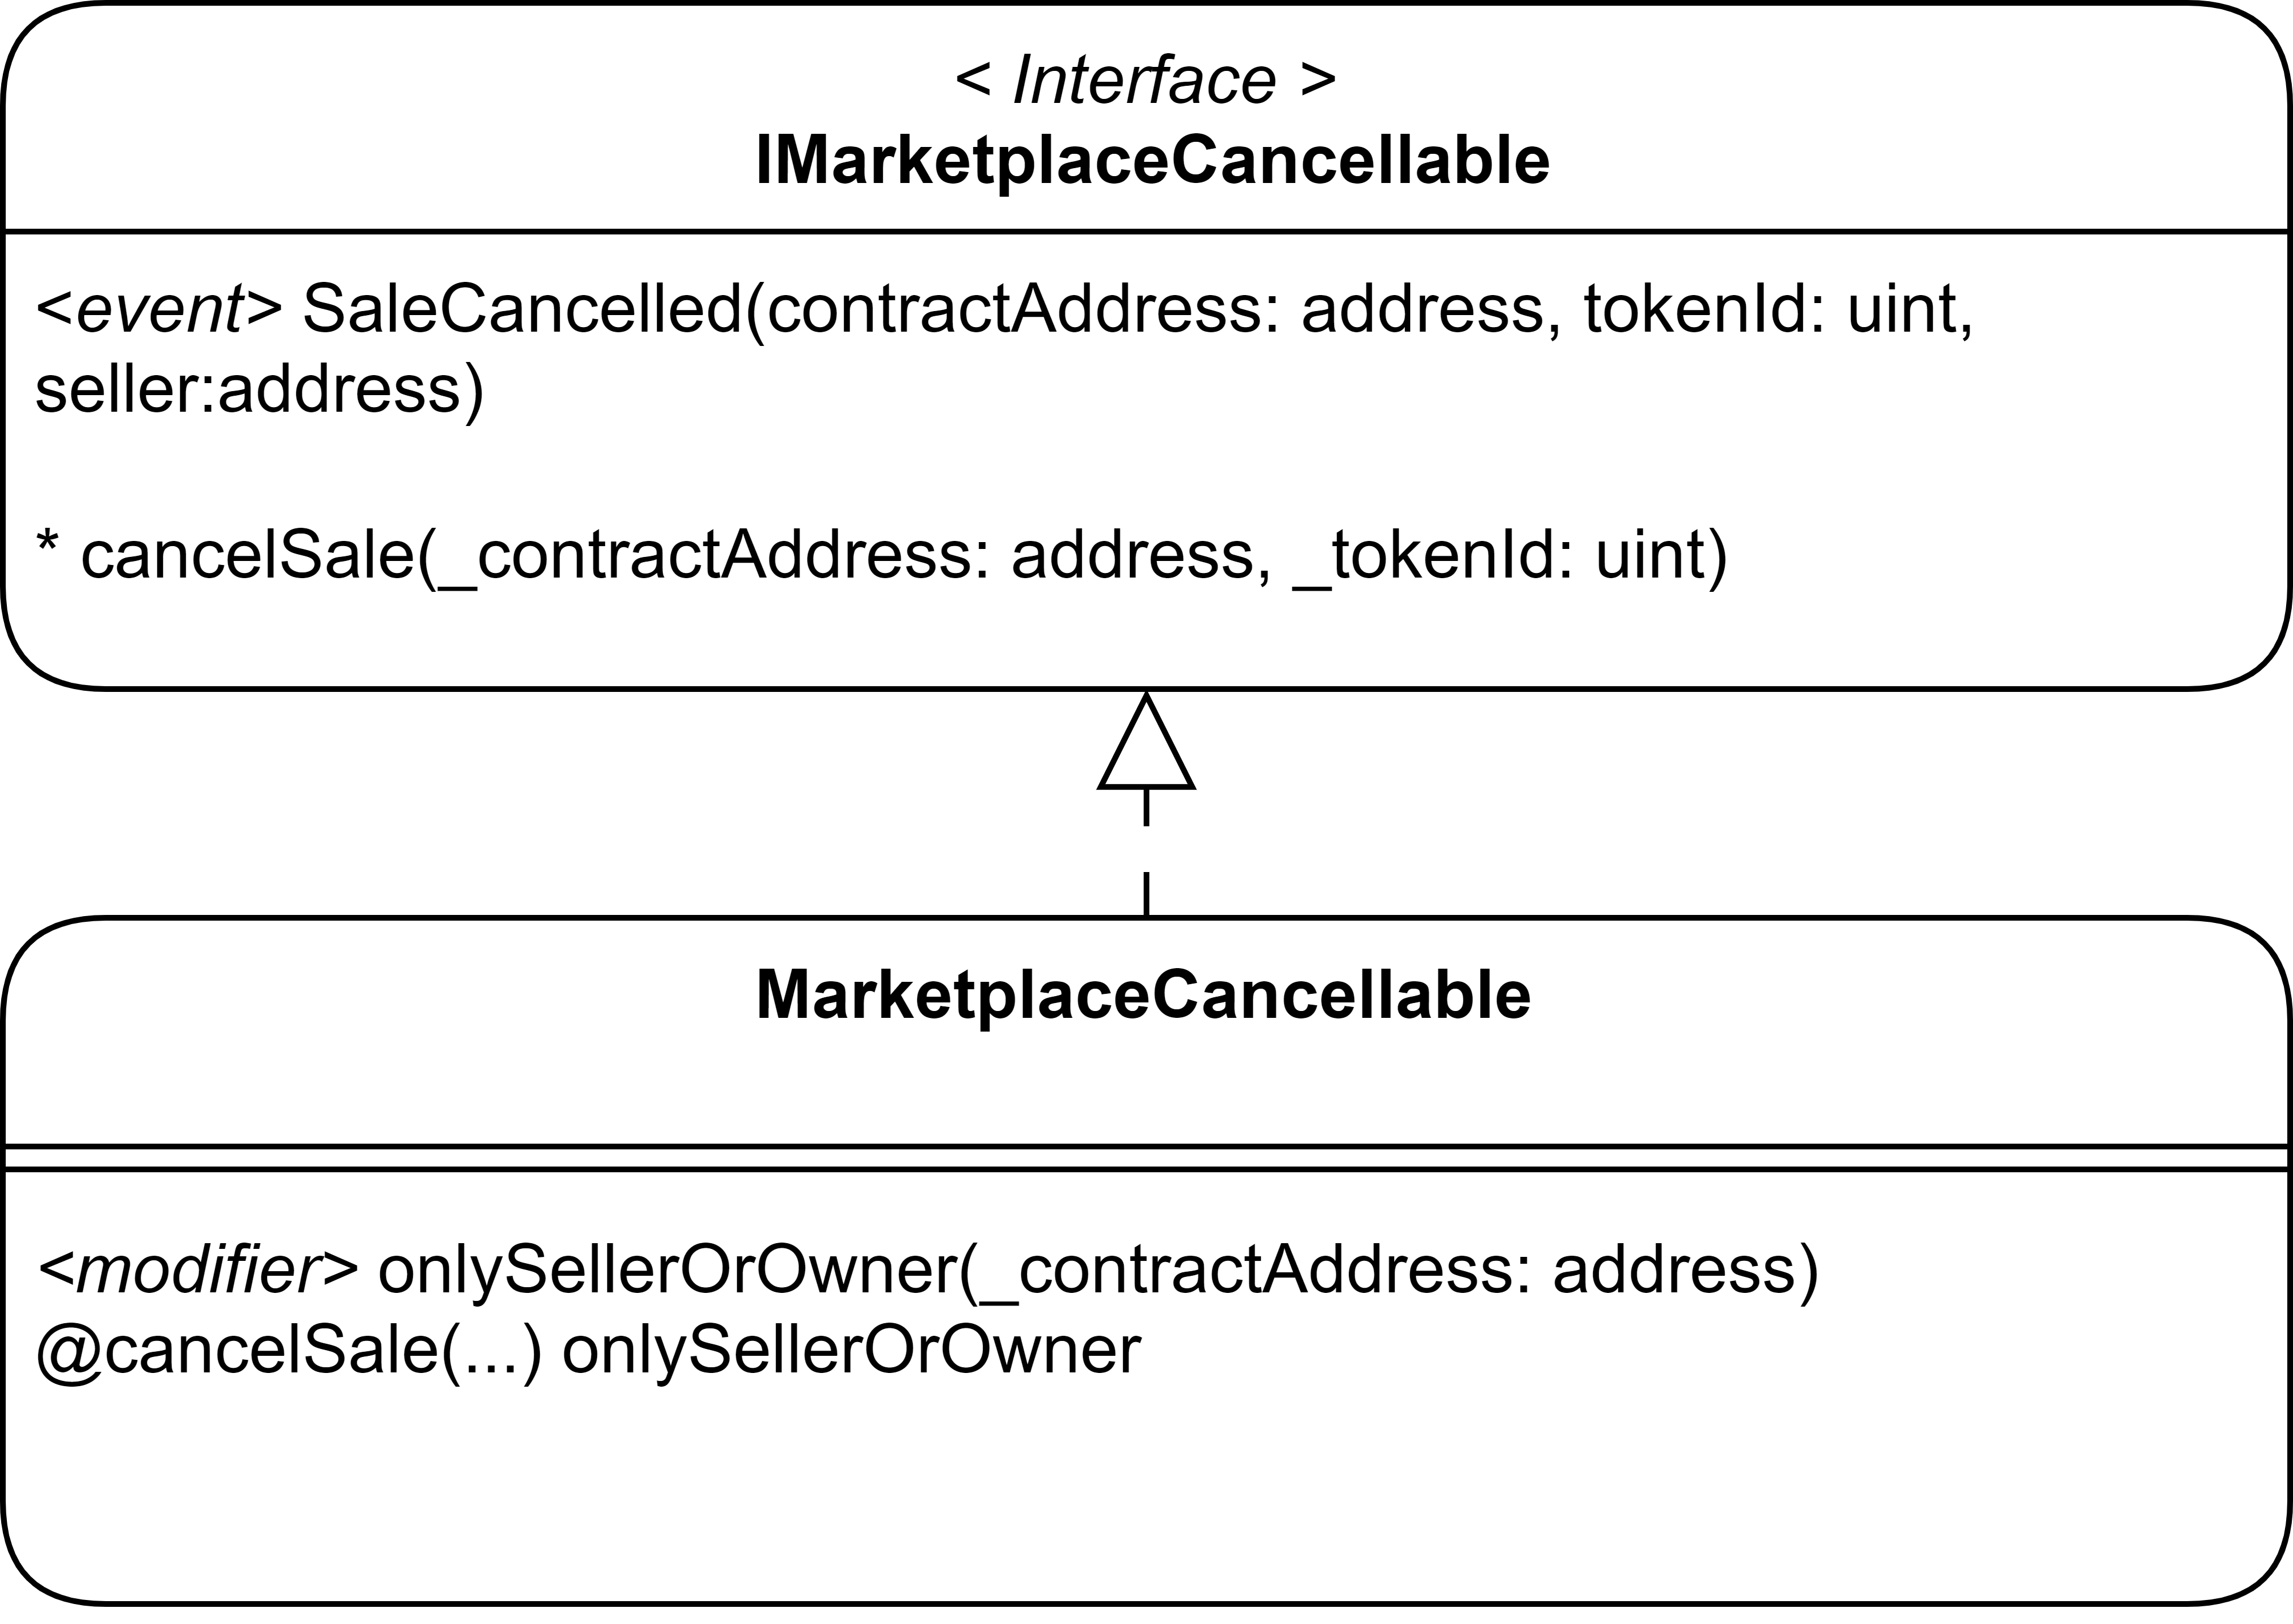
\includegraphics[width=0.7\textwidth]{images/blockchainContracts/MarketplaceCancellable.png}
    \caption{Marketplace Cancellable}
    \label{fig:marketplaceCancellable}
\end{figure}

\paragraph{Modifiable}
Il contratto \textit{MarketplaceModifiable} estende \textit{IMarketplaceModifiable} e \textit{IMarketplaceCancellable}. La sua funzione è quella di consentire la modifica del prezzo di vendita di un asset. Questa operazione è eseguibile unicamente dal possessore dell'asset, come visibile in figura \ref{fig:marketplaceModifiable}.

\begin{figure}[H]
    \centering
    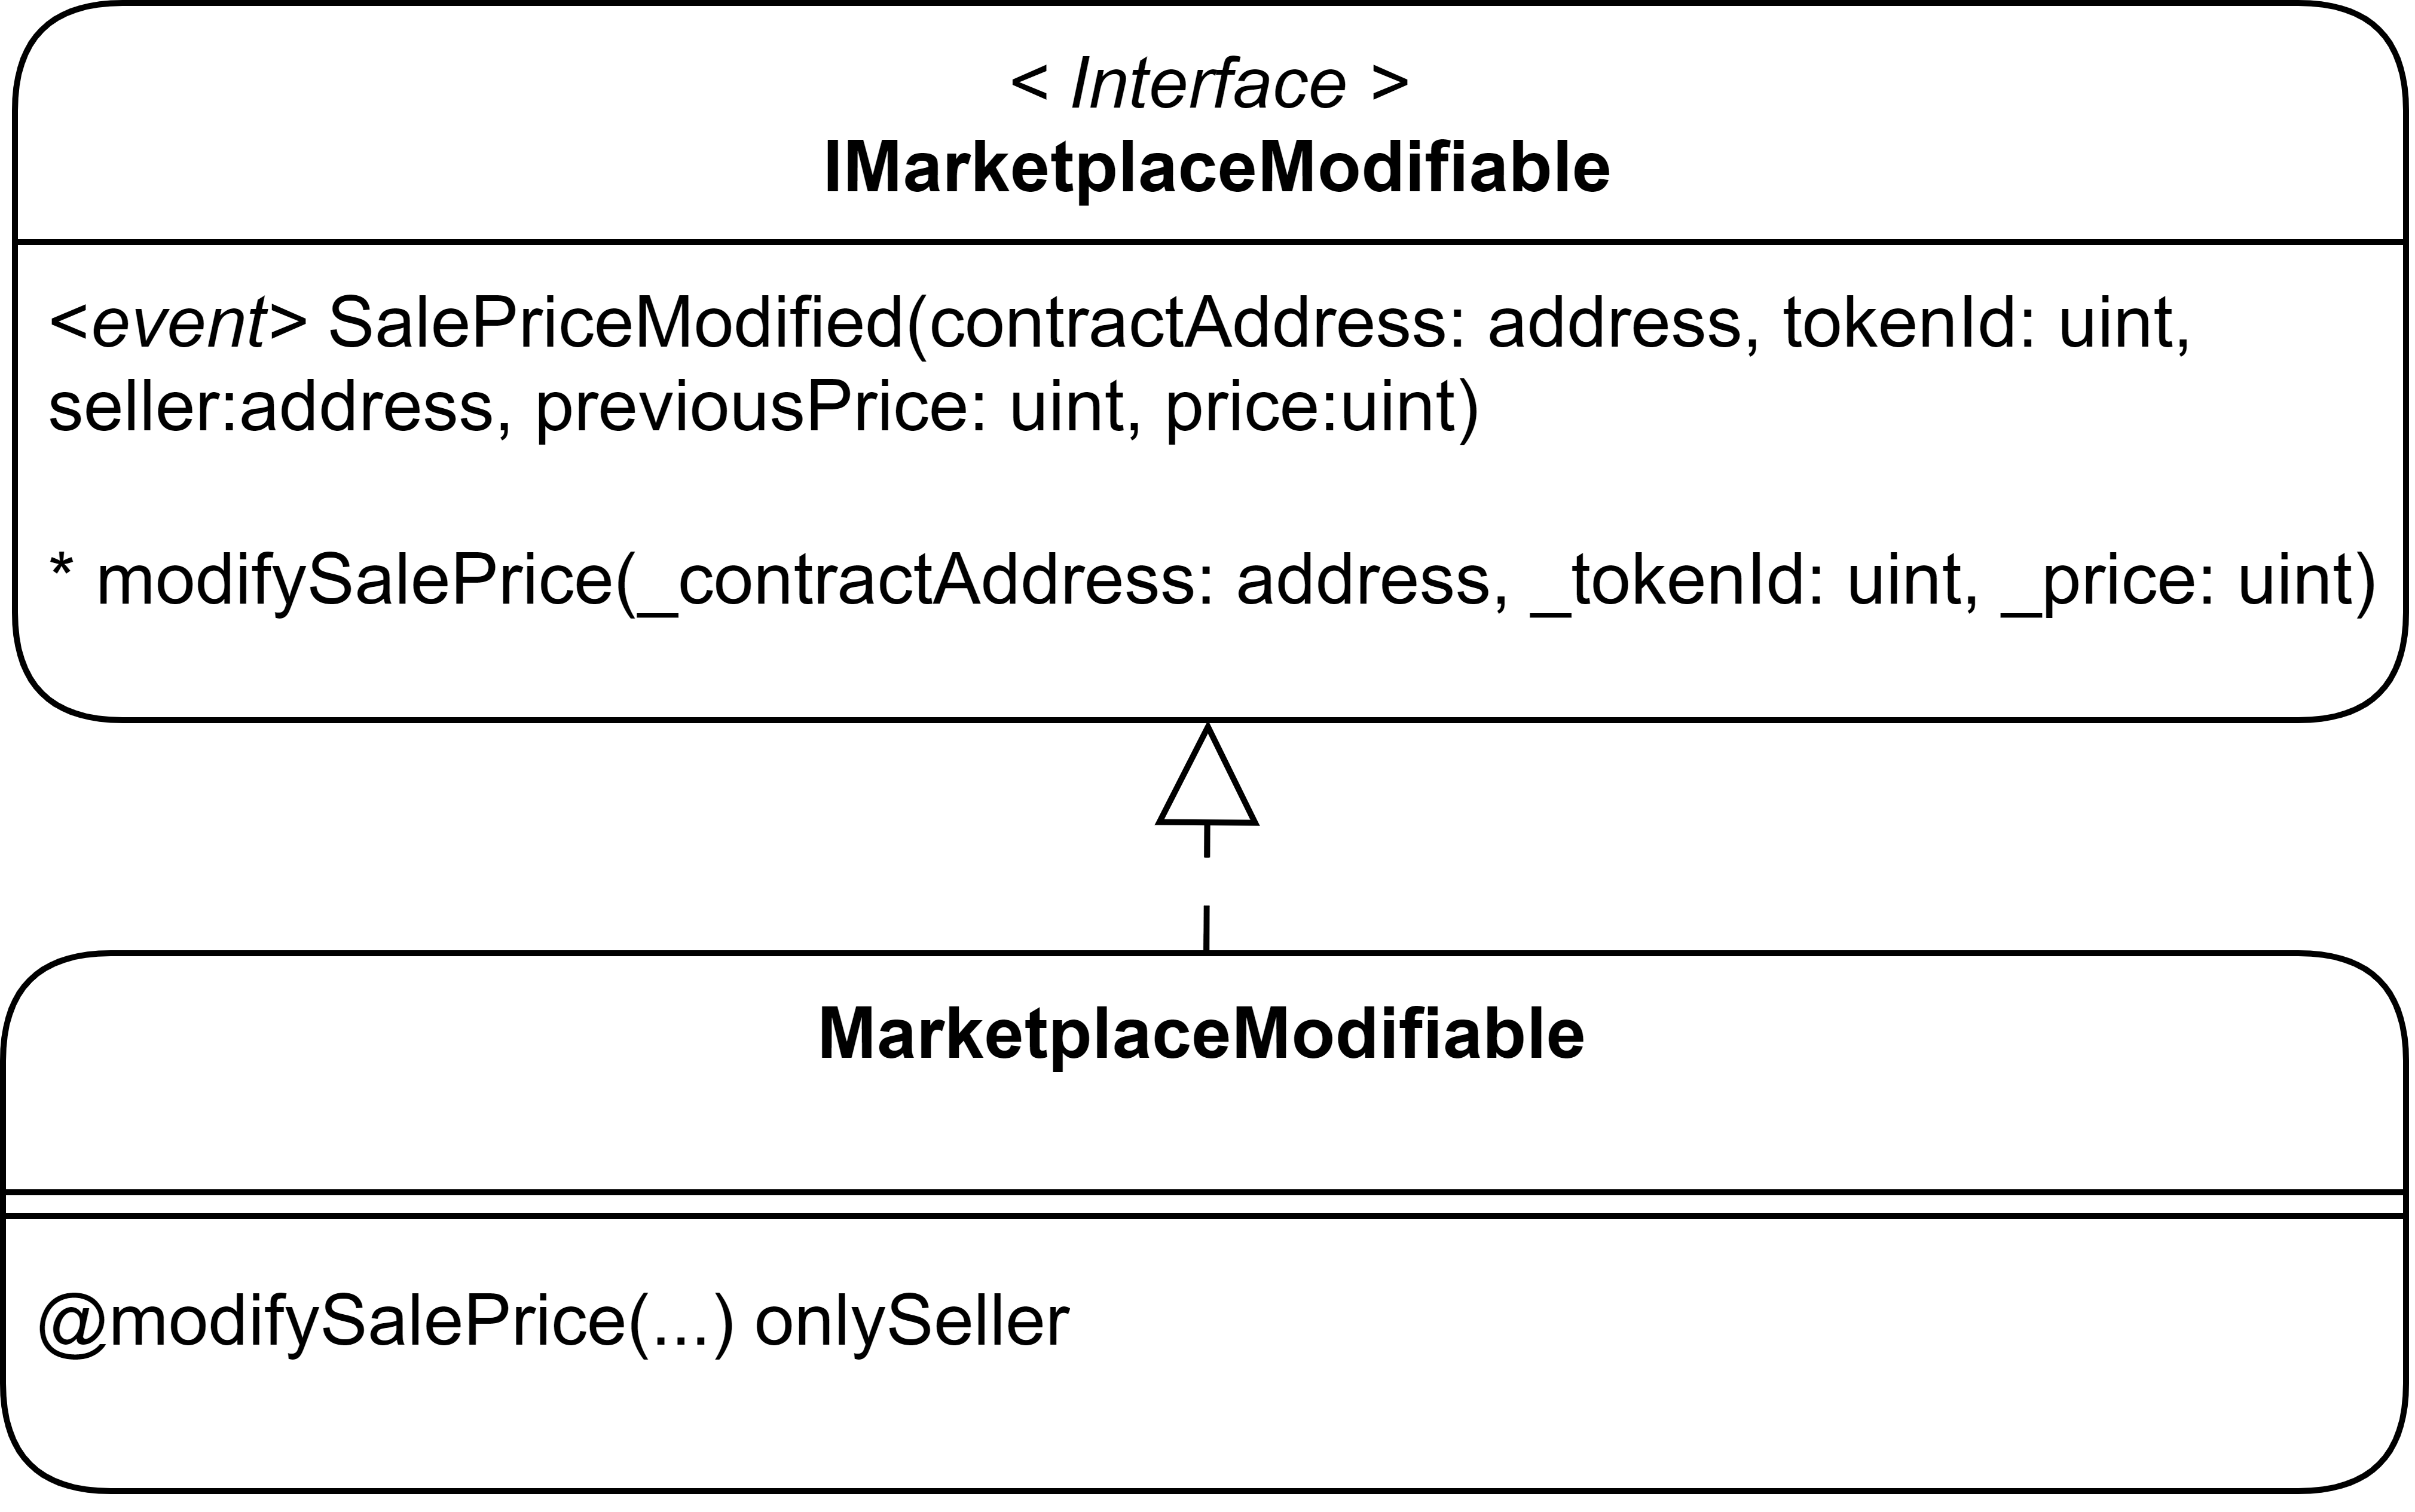
\includegraphics[width=0.7\textwidth]{images/blockchainContracts/MarketplaceModifiable.png}
    \caption{Marketplace Modifiable}
    \label{fig:marketplaceModifiable}
\end{figure}

\paragraph{Earnable}
\label{sec:marketplace-earnable}

Questo contratto consente il collezionamento di royalty a favore del marketplace per ogni acquisto effettuato. Come visibile in figura \ref{fig:marketplaceEarnable}, il contratto contiene il metodo \textit{receiver}, ovvero uno speciale metodo che permette al contratto di ricevere \textit{ETH}. La possibilità di collezionare le royalty è data dal metodo \textit{payShares}, il quale viene chiamato all'interno contratto \textit{MarketplaceFundamental}  nel momento in cui avviene un acquisto. 

Più in dettaglio, effettuando l'\textit{override} del metodo \textit{payShares}, che sarà chiamato dal metodo \textit{buy}, avviene una divisione del prezzo di vendita in base al valore presente nell'attributo \textit{royalty}. Questo valore rappresenta la percentuale di royalty che il marketplace riceverà per ogni acquisto, esso è un \textit{uint16} in quanto rappresenta un valore percentuale in \textit{basis point} (il valore 1 corrisponde allo 0.01\%, mentre il valore 10000 rappresenta il 100\%). In aggiunta, sono presenti alcune funzionalità di \textit{get} e \textit{set} per modificare il valore percentuale, nonchè diversi metodi per ritirare il saldo del contratto. 

\begin{figure}[H]
    \centering
    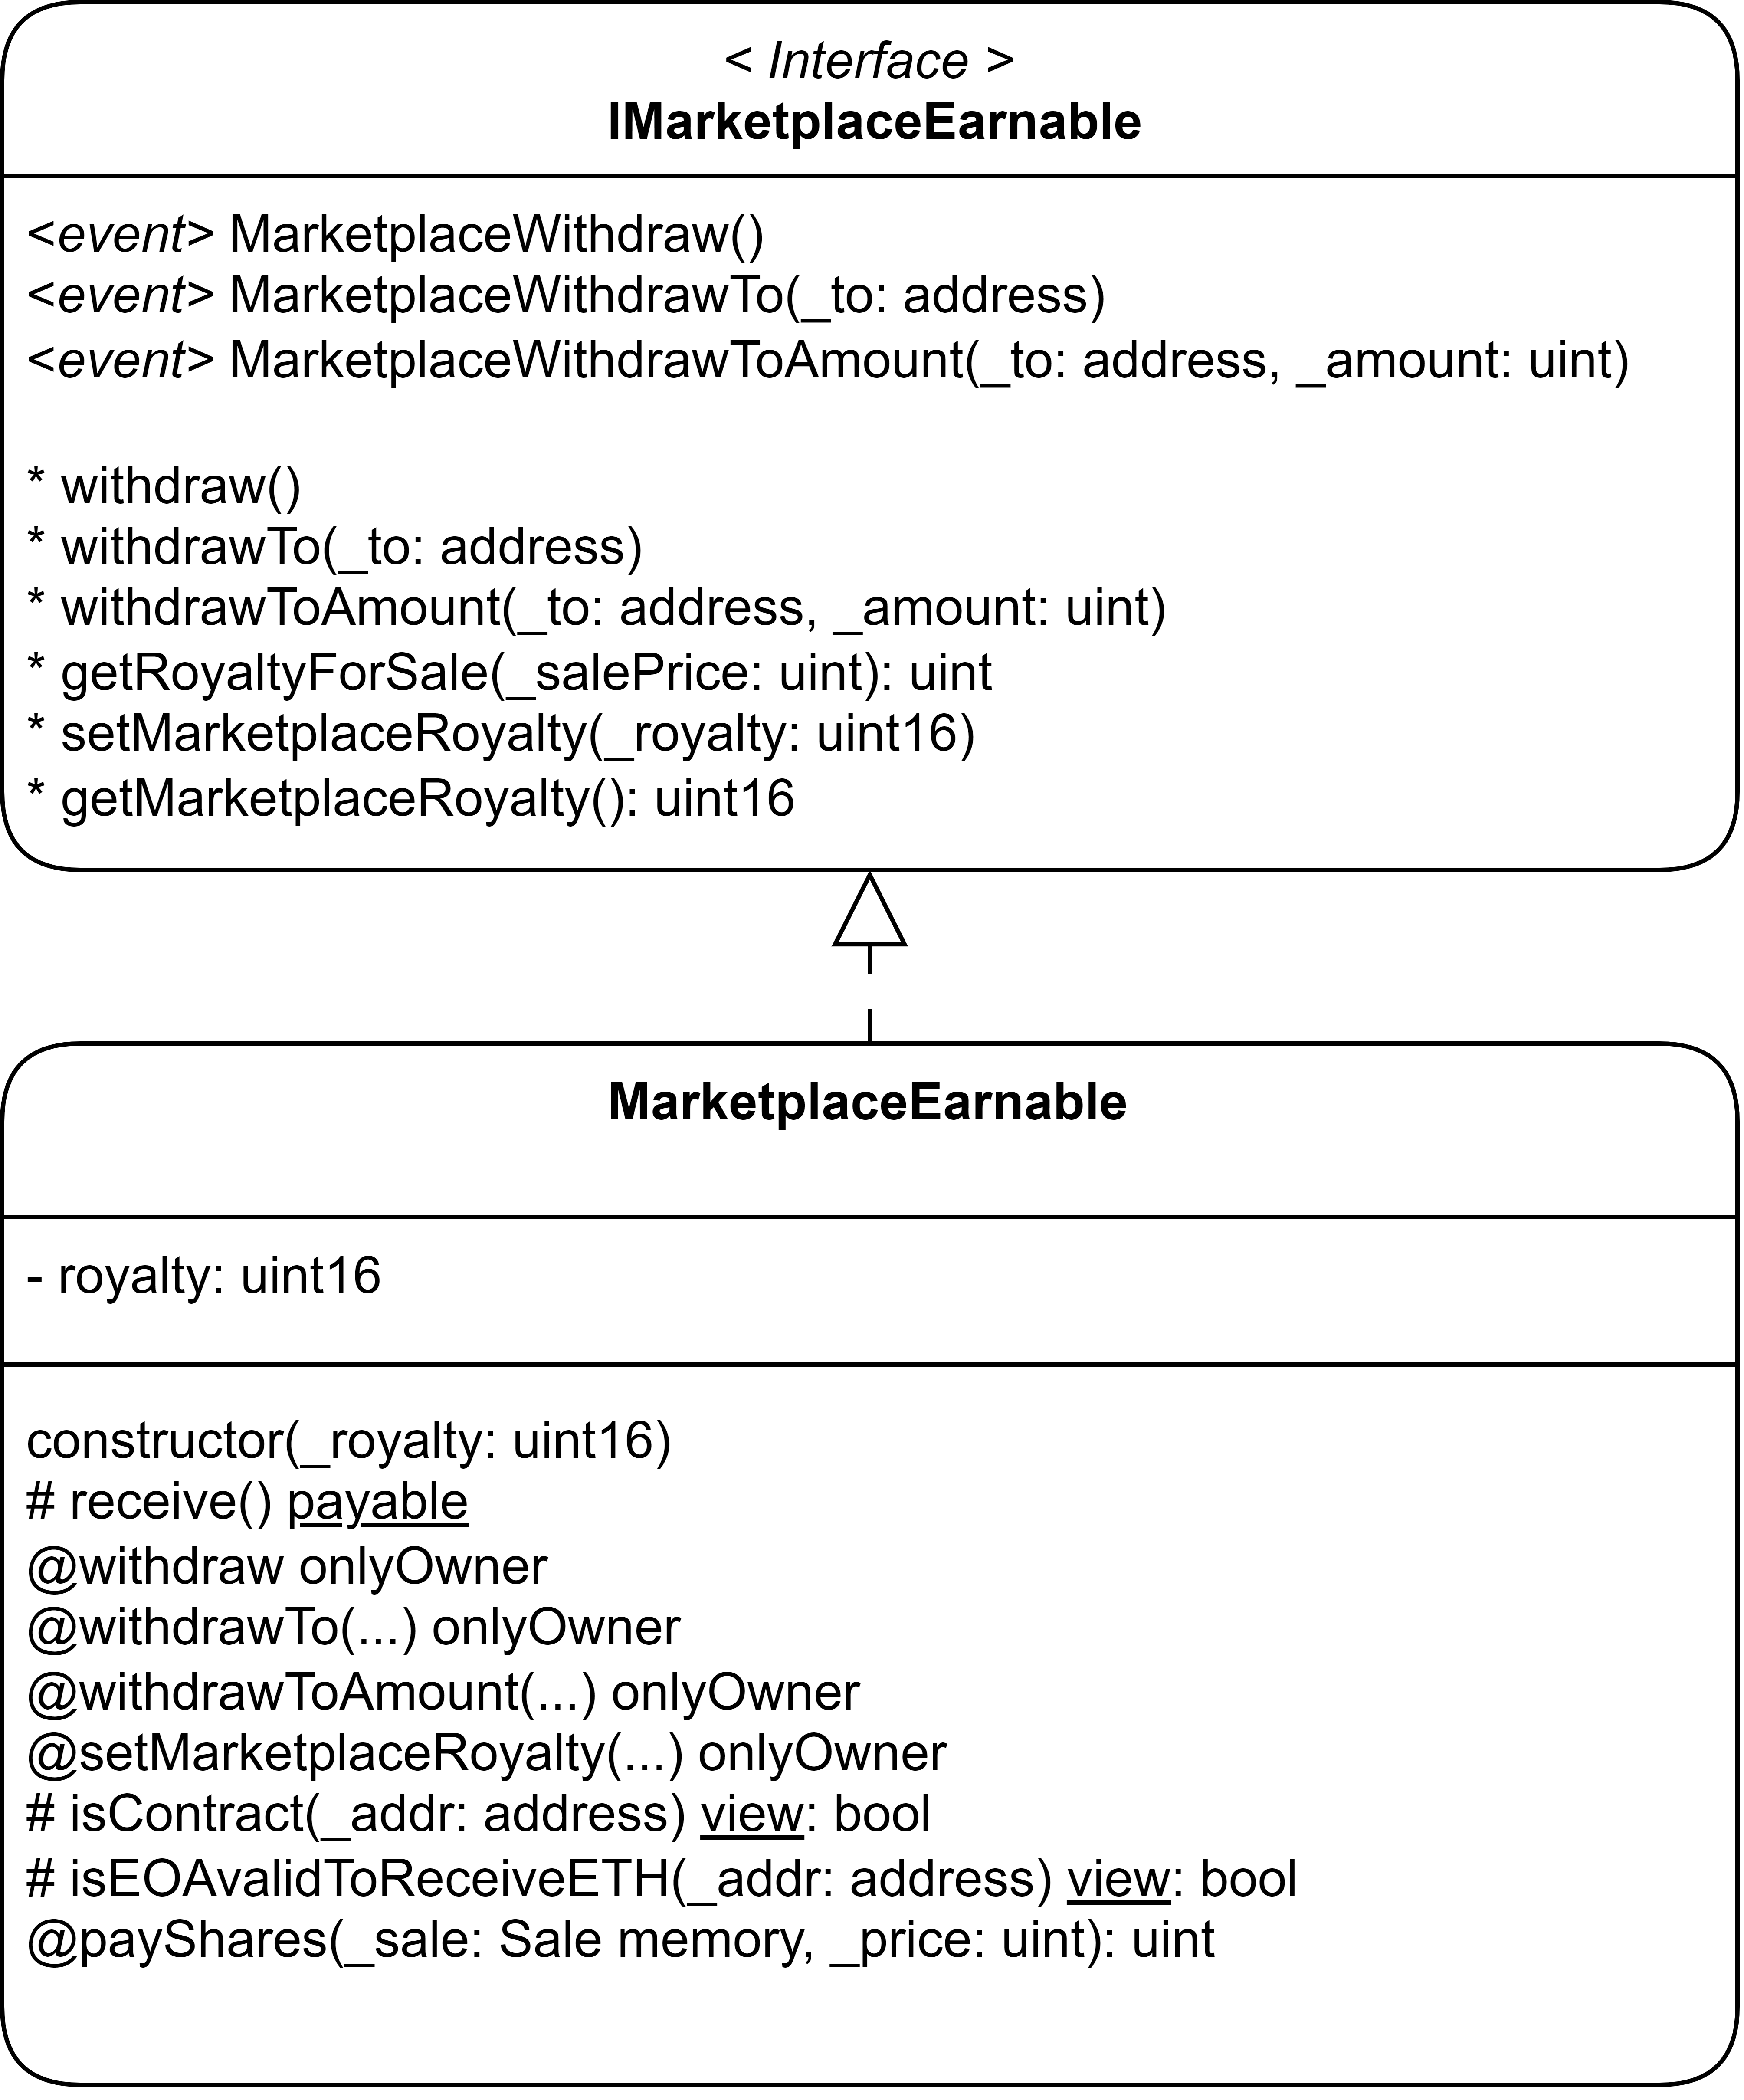
\includegraphics[width=0.7\textwidth]{images/blockchainContracts/MarketplaceEarnable.png}
    \caption{Marketplace Earnable}
    \label{fig:marketplaceEarnable}
\end{figure}

\paragraph{RoyaltyApplicable}
\label{sec:marketplace-royalty-applicable}

Il contratto \textit{RoyaltyApplicable} ha un funzionamento simile al contratto \hyperref[sec:marketplace-earnable]{\textit{Earnable}}. Ovvero, effettuando l'\textit{override} del metodo \textit{payShares} il saldo sarà diviso. In questo caso,
nel momento in cui avviene un acquisto il saldo inviato sarà separato tra il venditore e gli indirizzi definiti dal creatore dell'asset.

\begin{figure}[H]
    \centering
    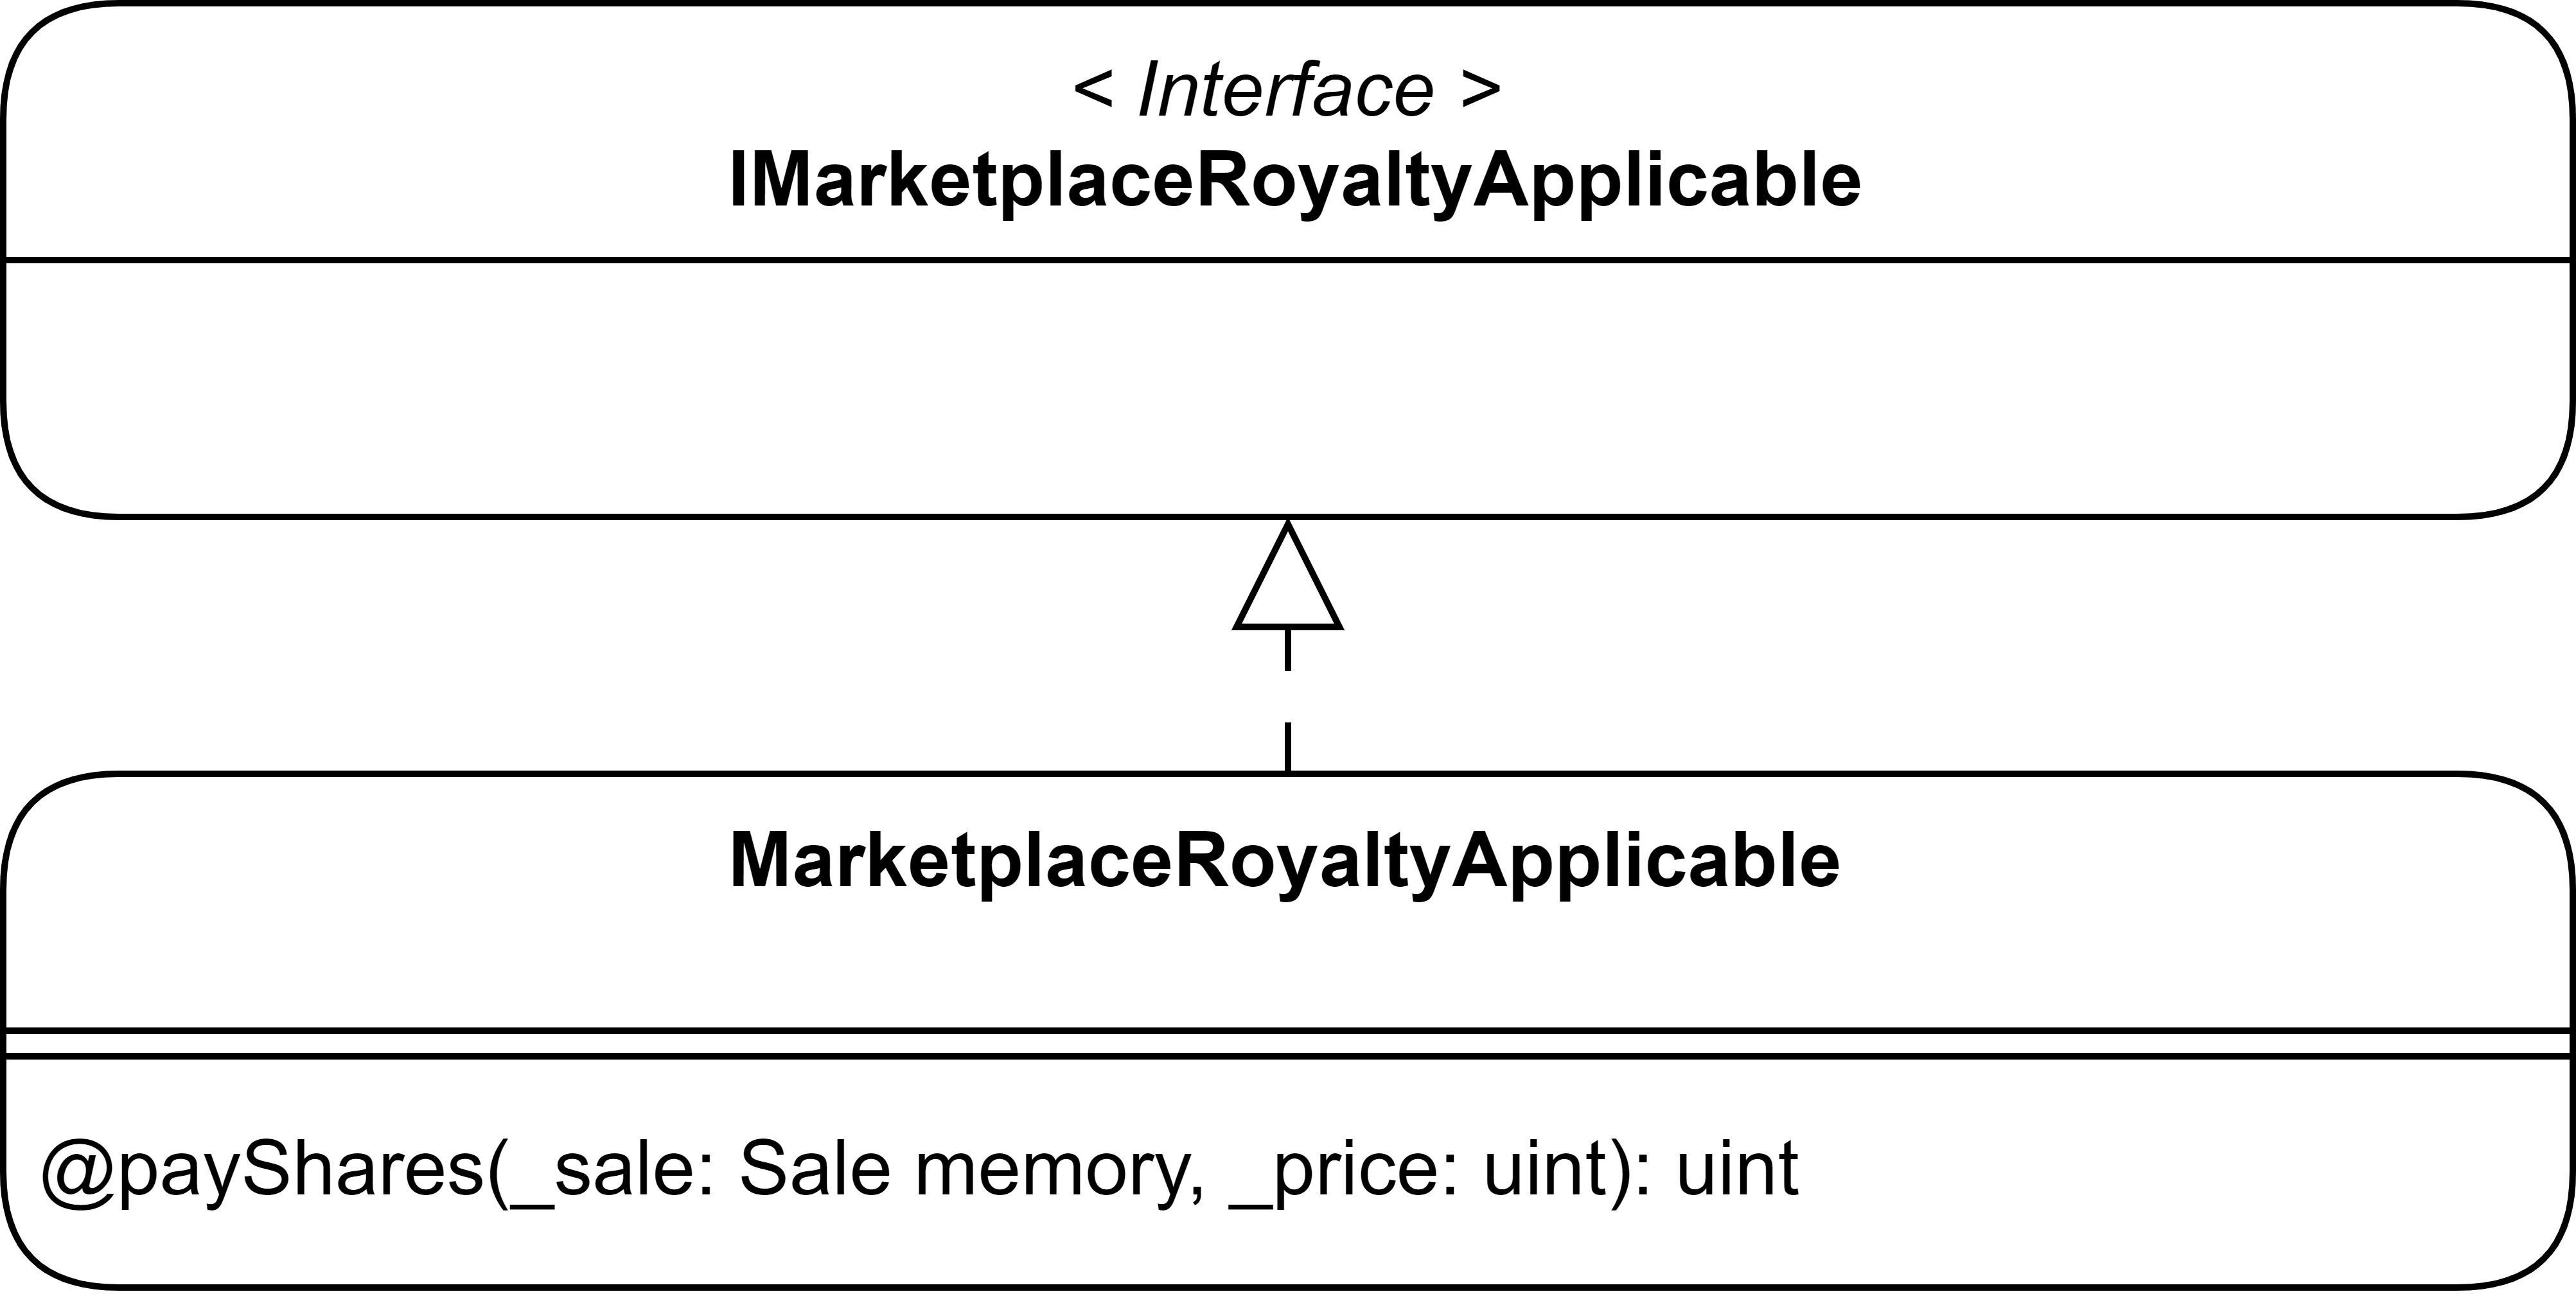
\includegraphics[width=0.7\textwidth]{images/blockchainContracts/MarketplaceRoyaltyApplicable.png}
    \caption{Marketplace RoyaltyApplicable}
    \label{fig:marketplaceRoyaltyApplicable}
\end{figure}


\paragraph{Cleanable}

All'interno del contratto \textit{Cleanable}, come rappresentato in figura \ref{fig:marketplaceCleanable}, sono presenti due metodi di gestione utilizzabili unicamente dall'amministratore, le loro funzionalità sono le seguenti:

\begin{itemize}
    \item \textit{cleanStorage}: Le informazioni relative a vendite cancellate o vendute rimangono all'interno del contratto. \textit{cleanStorage} permette di eliminare le informazioni relative a queste vendite allo scopo di ridurre la quantità di dati salvati all'interno del contratto, permettendo la riduzione dei tempi di attesa per l'esecuzione di alcune funzionalità sia \textit{on-chain} che \textit{off-chain}. Durante la progettazione del contratto è stato deciso di non cancellare queste informazioni all'acquisto, così da permettere agli utenti di risparmiare sulle \textit{gas fee}.
    \item \textit{cleanInqualities}: Questo metodo permette di eliminare le informazioni relative a vendite che non sono più corrette. Tale situazione può accadere nel momento in cui un utente trasferisce un asset in vendita esternamente al marketplace. In questo caso, la vendita rimarrebbe presente nel marketplace ma non sarebbe più valida. Un'alternativa per risolvere il problema è descritta nel capitolo \hyperref[sec:marketplace-royalty-applicable]{\textit{RoyaltyApplicable}}.
\end{itemize}

\begin{figure}[H]
    \centering
    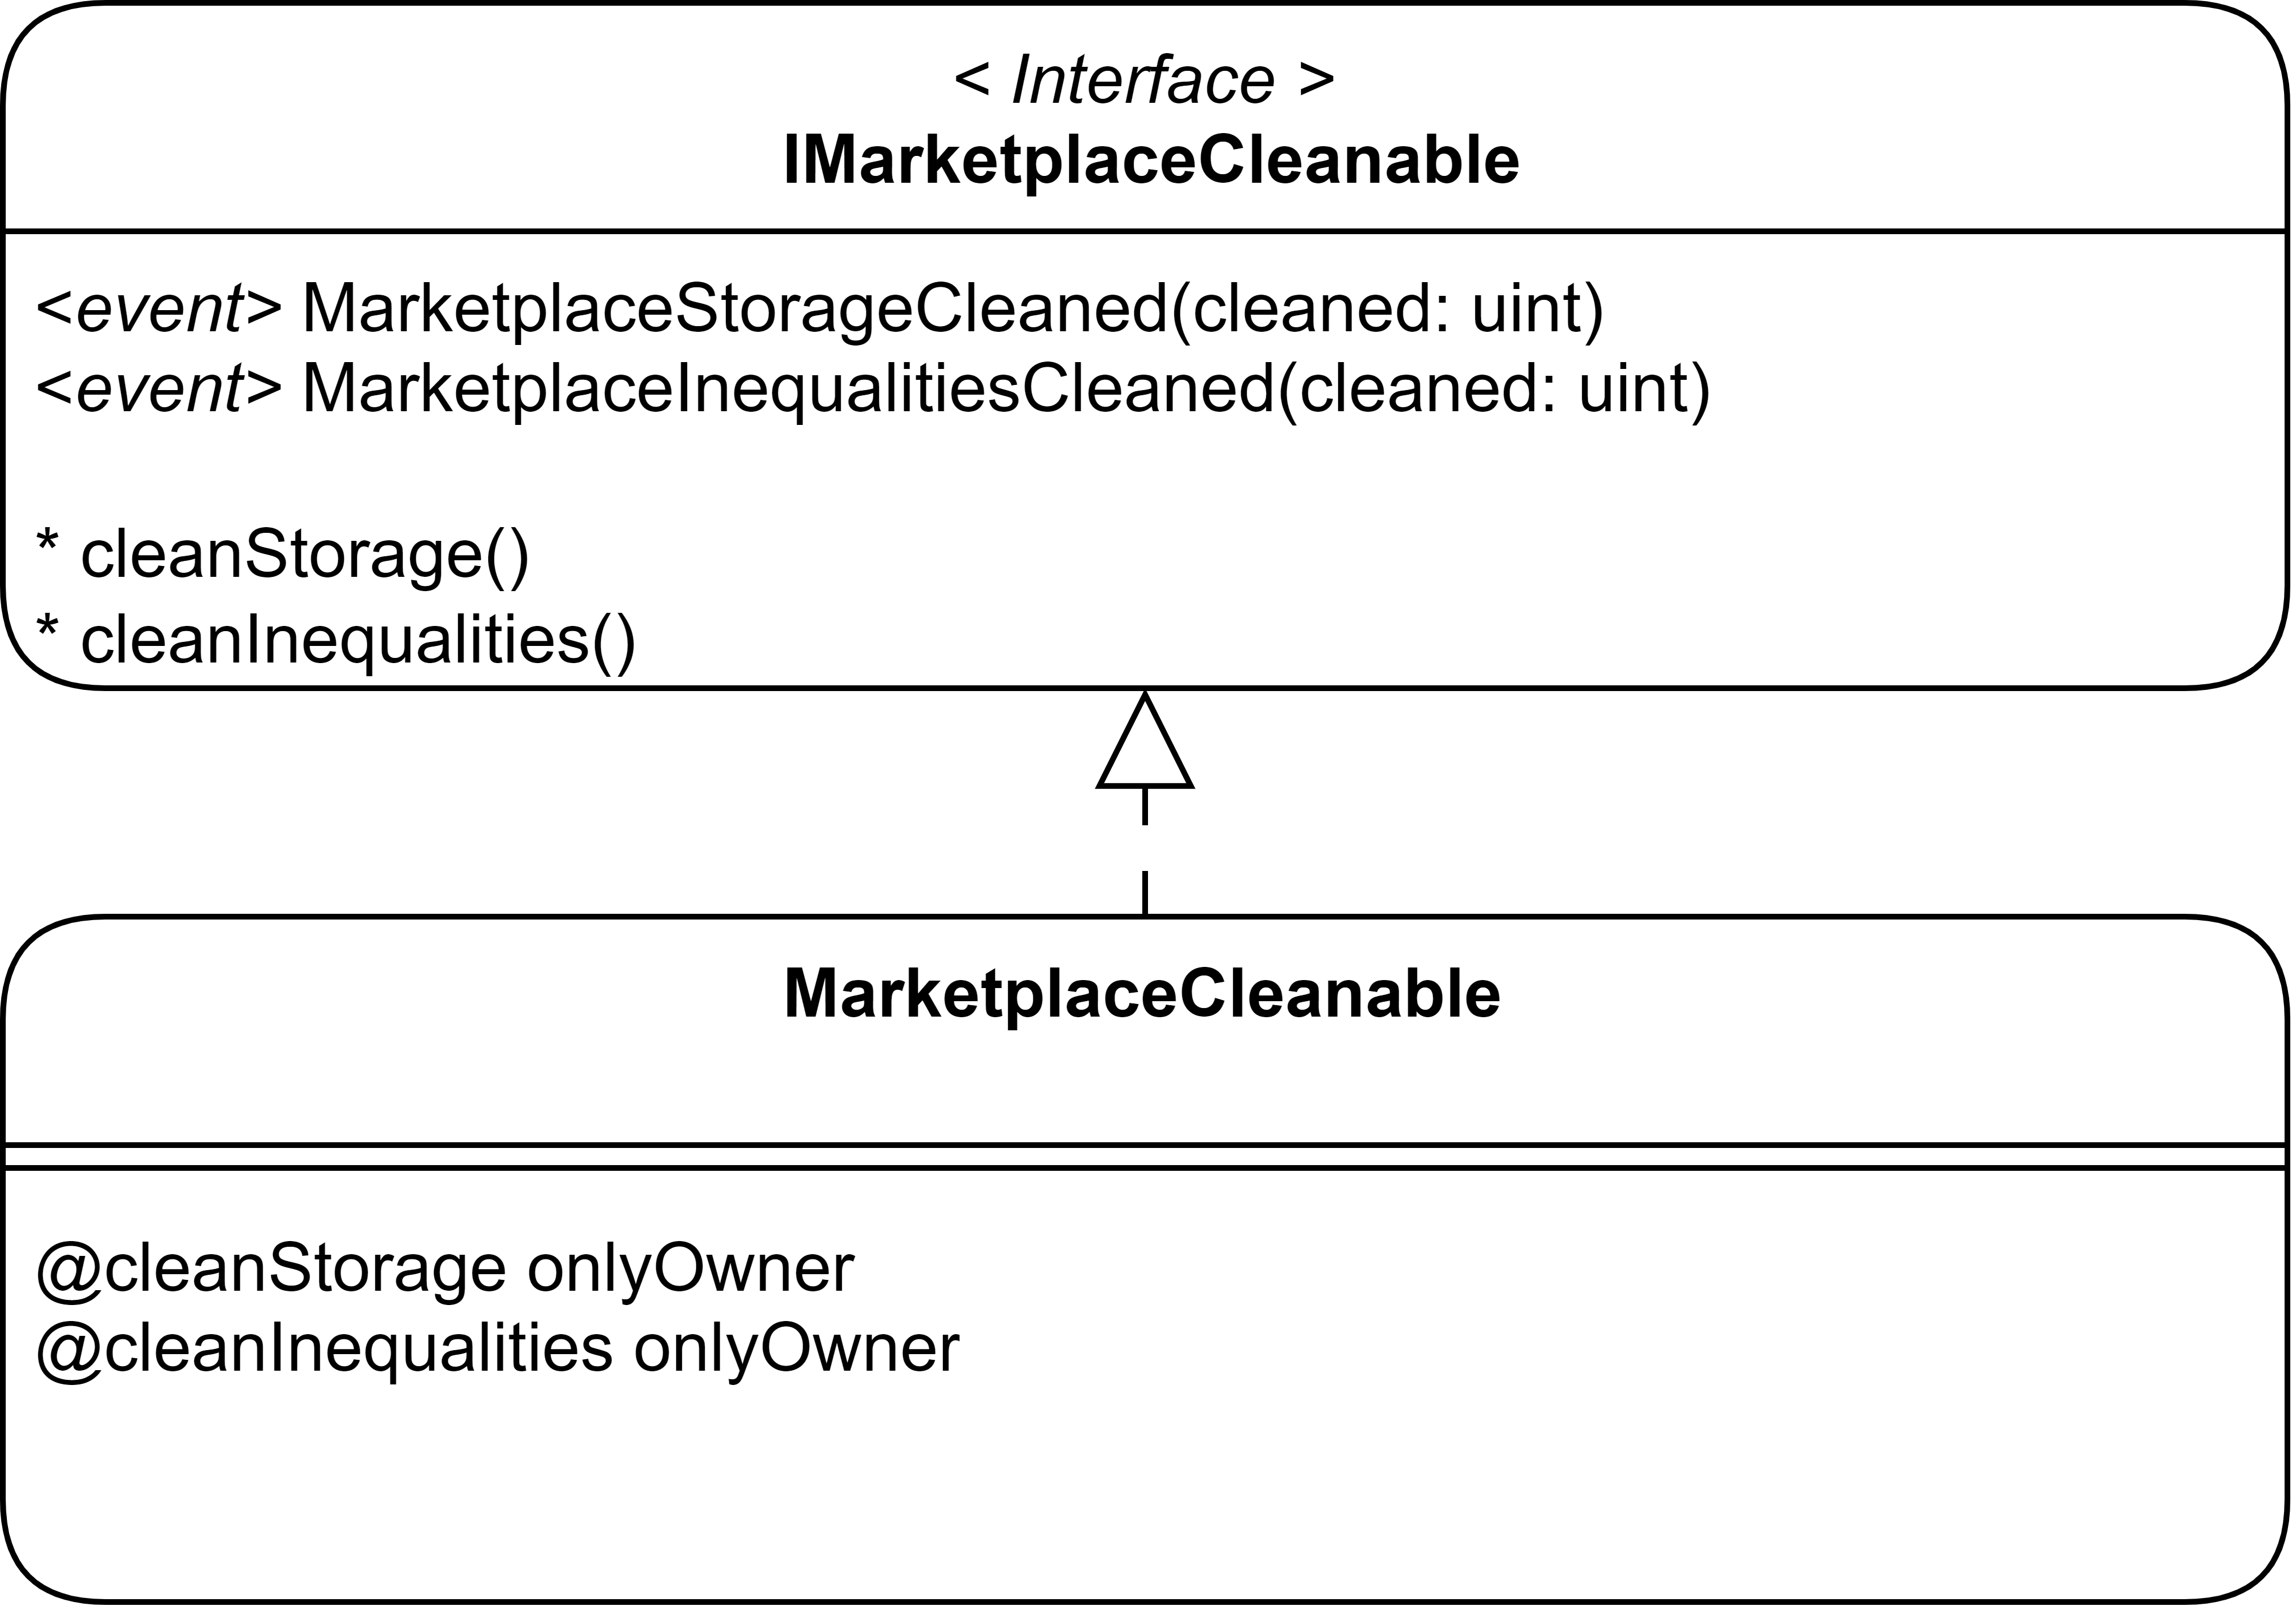
\includegraphics[width=0.7\textwidth]{images/blockchainContracts/MarketplaceCleanable.png}
    \caption{Marketplace Cleanable}
    \label{fig:marketplaceCleanable}
\end{figure}


\subsubsection{ERC721 Factory}

Come descritto nel capitolo \hyperref[sec:creazioneNFT]{\textit{Creazione NFT}}, l'utente ha tre possibilità per la generazione di un NFT, tra cui la creazione di una nuova collezione attraverso il \textit{depolyment} di un contratto ERC721. Per facilitare l'ultima operazione descritta, è stato sviluppato lo \textit{smart contract} \textit{ERC721 Factory}. Il quale permette di creare nuovi contratti utilizzando un \textit{template} chiamato \textit{Boilerplate ERC721}, analizzato nel prossimo capitolo. Come è possibile notare dalla figura \ref{fig:erc721Factory} il contratto presenta due metodi:

\begin{itemize}
    \item \textit{createERC721}: permette la creazione di un nuovo contratto ERC721, impostando un base URI per i metadati dei token (l'URI completo sarà composto da base URI + token ID), il nome e il simbolo della collezione. Inoltre, il metodo permette di impostare le \textit{royalties} di default per l'intero contratto e di effettuare l'operazione di \textit{mint} per un numero definito di asset.
    \item \textit{getAllERC721s}: questo metodo consente di ottenere tutti i contratti ERC721 creati attraverso la \textit{factory}. La sua utilità si presenta nel momento in cui l'utente vuole creare un nuovo NFT all'interno di una collezione già esistente. Infatti, filtrando in base all'\textit{owner} tutti i contratti ERC721, sarà possibile fornire all'utente unicamente quelli su cui ha il permesso di creare un nuovo NFT.
\end{itemize}

\begin{figure}[H]
    \centering
    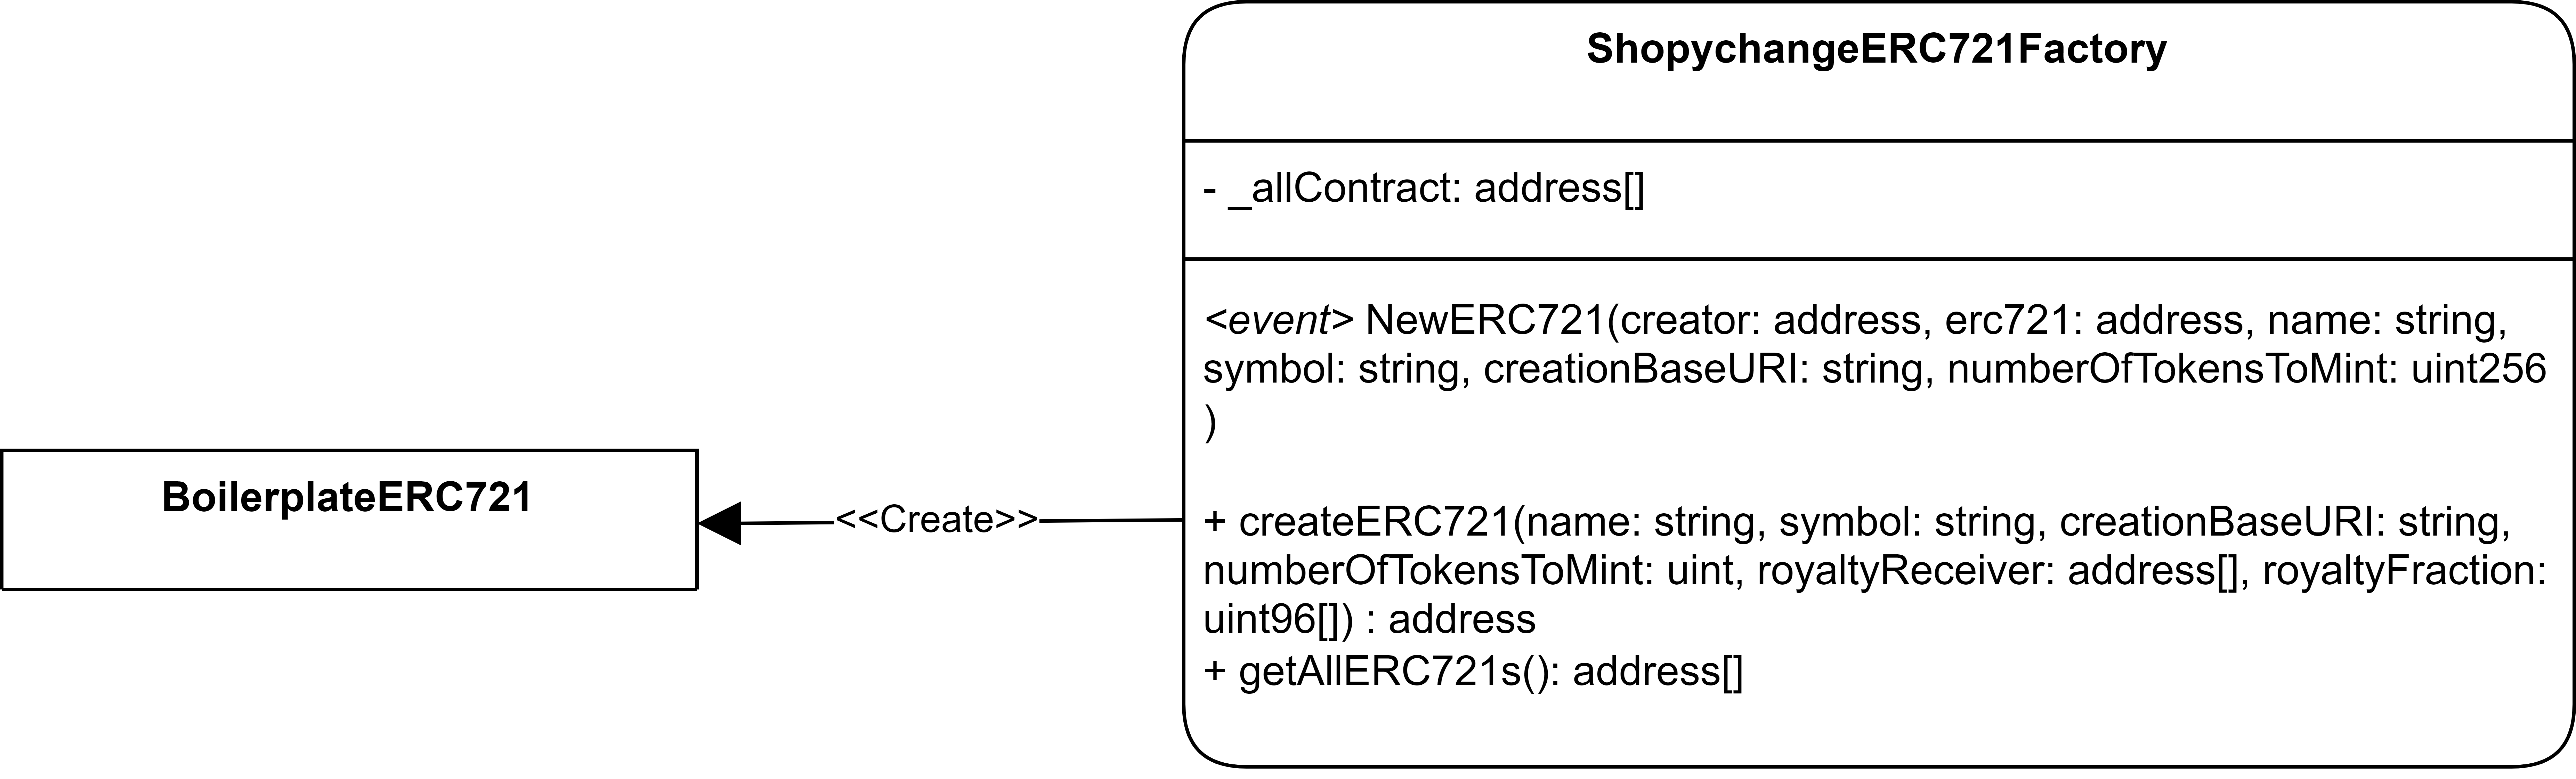
\includegraphics[width=0.7\textwidth]{images/blockchainContracts/ERC721Factory.png}
    \caption{ERC721 Factory}
    \label{fig:erc721Factory}
\end{figure}


\subsubsection{Boilerplate ERC721}

Il contratto \textit{Boilerplate ERC721} è un \textit{template} utilizzato per la creazione di nuovi contratti ERC721. Come visibile in figura \ref{fig:boilerplateERC721}, il contratto eredita da \textit{ERC721URIStorage}, \textit{ERC721Burnable} e \textit{ERC2981MultiReceiver}, questo permette di avere dei metadati per ogni token, di poter bruciare un token e di poter gestire le \textit{royalty} in maniera personalizzata.

\begin{figure}[H]
    \centering
    \includegraphics[width=0.7\textwidth]{images/blockchainContracts/BoilerplateERC721.png}
    \caption{BoilerplateERC721}
    \label{fig:boilerplateERC721}
\end{figure}

\paragraph{ERC2981MultiReceiver}
\label{sec:erc2981-multi-receiver}

Il contratto \textit{ERC2981MultiReceiver} è stato sviluppato per consentire la gestione delle \textit{royalty} in maniera personalizzata. 

Come visibile in figura \ref{fig:boilerplateERC721}, il contratto eredita da \textit{IERC2981Royalties}, il quale definisce le funzionalità obbligatorie per la gestione delle \textit{royalties}.

Come descritto più in dettaglio nel capitolo \hyperref[sec:utilizzo-erc2981-payment-splitter]{\textit{Utilizzo di ERC2981 e PaymentSplitter}} il contratto \textit{ERC2981MultiReceiver} è stato creato per poter gestire le \textit{royalties} con più di un ricevente. Infatti, già nel momento di creazione di un nuovo contratto \textit{BoilerplateERC721}, nel caso in cui vengano specificati più indirizzi, avverrà la creazione di un \textit{PaymentSplitter} di default. In questo modo, nel momento in cui avviene un acquisto, il saldo verrà diviso in base alla percentuale definita per ogni indirizzo. In aggiunta, il contratto permette la creazione di \textit{royalty} personalizzate per ogni token, creando contratti \textit{PaymentSplitter} all'occorenza.

\paragraph{PaymentSplitter}

Il contratto \textit{PaymentSplitter} offre la possibilità di dividere il saldo in base alla percentuale definita per ogni indirizzo. Nel momento in cui avviene un acquisto, il marketplace, o più specificamente il contratto \hyperref[sec:marketplace-royalty-applicable]{\textit{RoyaltyApplicable}}, invierà il saldo relativo alle \textit{royalties} al contratto \textit{PaymentSplitter}. Tuttavia, a causa di una limitazione implementativa del metodo \textit{receiver}, sarà compito dei riceventi di recupare il saldo ottenuto, l'operazione è possibile tramite il metodo \textit{release}. All'interno del capitolo \hyperref[sec:revenue-share]{\textit{Revenue Share}} è possibile osservare un esempio di utilizzo del contratto \textit{PaymentSplitter}.

\subsubsection{Storage}
Il contratto storage è semplicemente un contratto \textit{BoilerplateERC721} con la particolarità che chiunque può effettuare l'operazione di \textit{mint}. Esso è stato sviluppato per permettere a tutti glii utenti di creare un singolo asset senza la necessità di creare una collezione. 

\subsection{Scripts}

Per le operazioni di distribuzione dei contratti sono stati creati degli script appositi, i quali permettono l'automazione di alcuni processi ripetitivi.

Lo script chiamato \textit{copyArtifacts} permette di copiare gli artefatti generati dalla compilazione degli smart contracts in una cartella definita.

Lo script \textit{modifyEnv} ha lo scopo di modificare i file \textit{.env}, ovvero i file di configurazione presenti sia nel frontend che nel backend. Più in dettaglio, questo script permette di modificare il valore di variabili definite con uno nuovo. Il suo utilizzo è molto utile nel momento in cui si effettua il \textit{deploy} di un contratto. Infatti, il contratto appena distribuito avrà un indirizzo diverso rispetto a quello precedente ed è quindi necessario modificare i file di \textit{envirorment} per permettere al frontend e al backend di interagire con il nuovo contratto.

Infine, è stato creato uno script chiamato \textit{deployAll}, esso permette di distrubito tutti i contratti sopracitati aggiornando gli artefatti e modificando i file \textit{.env}.

\subsection{Test}

Per verificare il corretto funzionamento degli smart contracts sono stati sviluppati dei test utilizzando la libreria \textit{ethers}, già presente nel framework \textit{Hardhat}. I test effettuati sono di due tipi: \textit{unit test} e \textit{integration test}.
I primi si occupano di verificare il corretto funzionamento di una singola funzionalità all'interno di un contratto. Mentre i secondi, si occupano di verificare il corretto funzionamento di più funzionalità all'interno di più contratti oppure di un singolo contratto generato ereditando più moduli, come nel caso del contratto \textit{ShopychangeMarketplace}.

\subsection{Motivazioni e Alternative}

La scelta che ha portato all'utilizzo di \textit{Hardhat} è stata fatta in quanto è un framework molto utilizzato e ben documentato, inoltre permette di creare un'istanza di un nodo locale, così da poter utilizzare una blockchain locale rendendo più semplice lo sviluppo e i test dell'intera applicazione. Per quanto riguarda la scelta del linguaggio di programmazione, è stato deciso di utilizzare \textit{Solidity} in quanto è il linguaggio più utilizzato per lo sviluppo di smart contracts. Inoltre, è possibile trovare una vasta documentazione e numerosi esempi di codice. 

In aggiunta, Durante lo svolgimento del progetto è stato utilizzato anche il webtool \textit{Remix}, il quale permette di scrivere, compilare e distribuire gli \textit{smart contracts}. In aggiunta, \textit{Remix} ha la funzionalità di poter interagire con gli \textit{smart contracts} attraverso dei semplici pulsanti, velocizzando l'interazione.

Inoltre, durante la fase di sviluppo è stato deciso di non utilizzare \textit{Typechain}, il quale permette di generare dei tipi TypeScript a partire dagli smart contracts. Questa scelta è stata fatta in quanto la libreria di interazione con i contratti a livello frontend (\textit{wagmi}) non supporta i tipi generati da \textit{Typechain}. Tuttavia, è possibile utilizzare \textit{Typechain} in combinazione con \textit{ethers} (una libreria largamente utilizzata per l'interazione con gli smart contracts).

Le alternative in ambito implementativo sono molteplici, così come le tecnologie utilizzabili. In particolare, per lo sviluppo degli smart contracts è possibile utilizzare diversi linguaggi di programmazione, tra cui \textit{Solidity}, \textit{Vyper} e \textit{Fe}. Anche i framework utilizzabili sono numerosi, tra cui \textit{Hardhat}, \textit{Truffle}\footnote{https://trufflesuite.com/} e \textit{Embark}\footnote{https://framework.embarklabs.io/}.